\documentclass[12pt,a4paper]{article}

% --- PAKIETY ---
\usepackage[utf8]{inputenc}
\usepackage[T1]{fontenc}
\usepackage[polish]{babel}
\usepackage{graphicx}      % Wstawianie wykresów
\usepackage{geometry}      % Ustawienia marginesów
\usepackage{amsmath}       % Matematyka
\usepackage{times}         % Czcionka sprawozdawcza
\usepackage{float}         % Wymuszanie pozycji obrazków (parametr H)
\usepackage{booktabs}

% Ustawienia marginesów
\geometry{margin=2cm}

\begin{document}

% --- NAGŁÓWEK ---
\noindent
\begin{minipage}[t]{0.5\textwidth}
    \begin{flushleft}
        Filip Graczyk, 254757 \\
        Filip Szymala, 254882
    \end{flushleft}
\end{minipage}
\begin{minipage}[t]{0.5\textwidth}
    \begin{flushright}
        Środa, 10:00 \\
        \today
    \end{flushright}
\end{minipage}

\vspace{1cm}

\begin{center}
    {\Large \textbf{Sztuczna inteligencja i systemy ekspertowe}} \\
    \vspace{0.2cm}
    {\large Zadanie 1: Piętnastka}
\end{center}

\vspace{1cm}

% --- CEL ---
\section{Cel}
Implementacja algorytmów przeszukiwania przestrzeni stanów (BFS, DFS oraz A*) w celu rozwiązania układanki „Piętnastka” oraz przeprowadzenie badań ich efektywności. Analiza skupia się na porównaniu wpływu parametrów algorytmów, takich jak porządek przeszukiwania sąsiedztwa i rodzaje heurystyk, na jakość uzyskanych rozwiązań oraz złożoność obliczeniową procesów.

% --- WYNIKI ---
\section{Wyniki}
Program został zaimplementowany w języku \textbf{Python} w wersji 3.14.0.

\subsection{Kryterium 1: Długość znalezionego rozwiązania}
\begin{figure}[H]
    \centering
    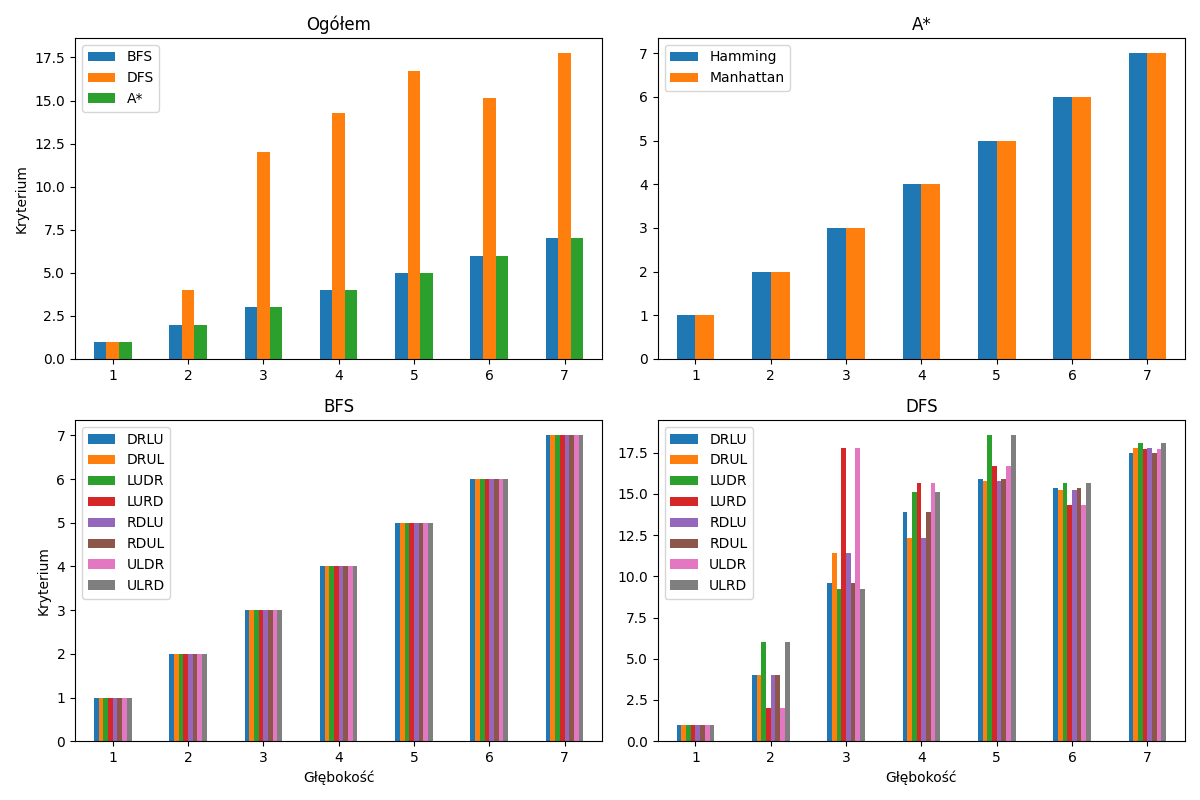
\includegraphics[width=0.9\textwidth]{wyniki_dlugosc.png}
    \caption{Długość znalezionego rozwiązania w zależności od głębokości stanu początkowego.}
\end{figure}

\subsection{Kryterium 2: Liczba stanów odwiedzonych}
\begin{figure}[H]
    \centering
    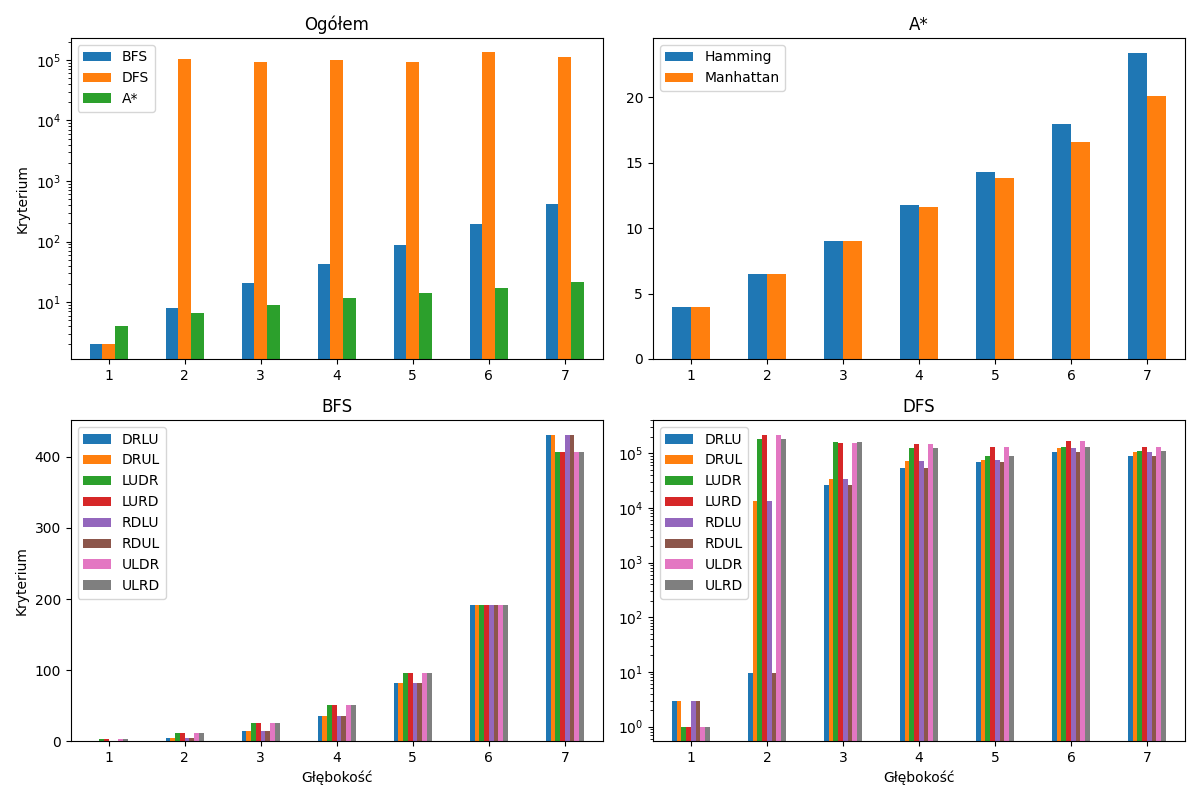
\includegraphics[width=0.9\textwidth]{wyniki_odwiedzone.png}
    \caption{Liczba stanów odwiedzonych w zależności od głębokości stanu początkowego.}
\end{figure}

\subsection{Kryterium 3: Liczba stanów przetworzonych}
\begin{figure}[H]
    \centering
    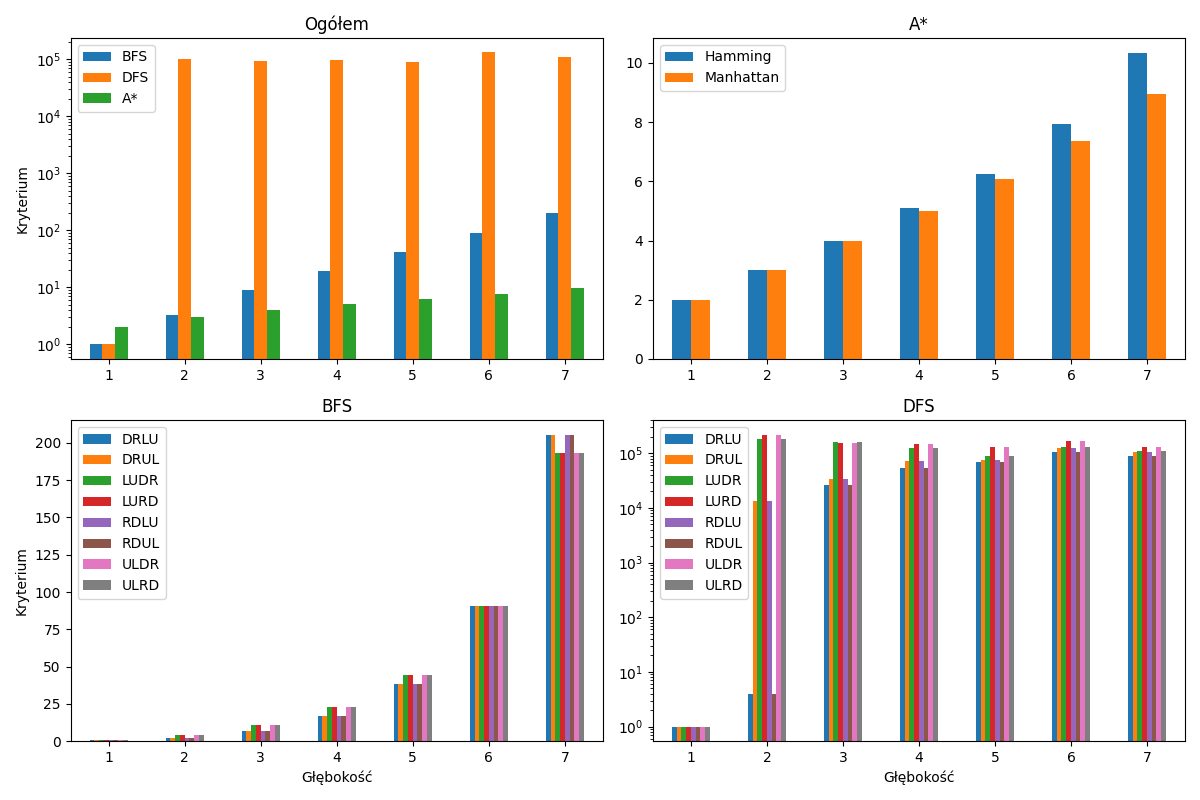
\includegraphics[width=0.9\textwidth]{wyniki_przetworzone.png}
    \caption{Liczba stanów przetworzonych w zależności od głębokości stanu początkowego.}
\end{figure}

\subsection{Kryterium 4: Maksymalna osiągnięta głębokość rekursji}
\begin{figure}[H]
    \centering
    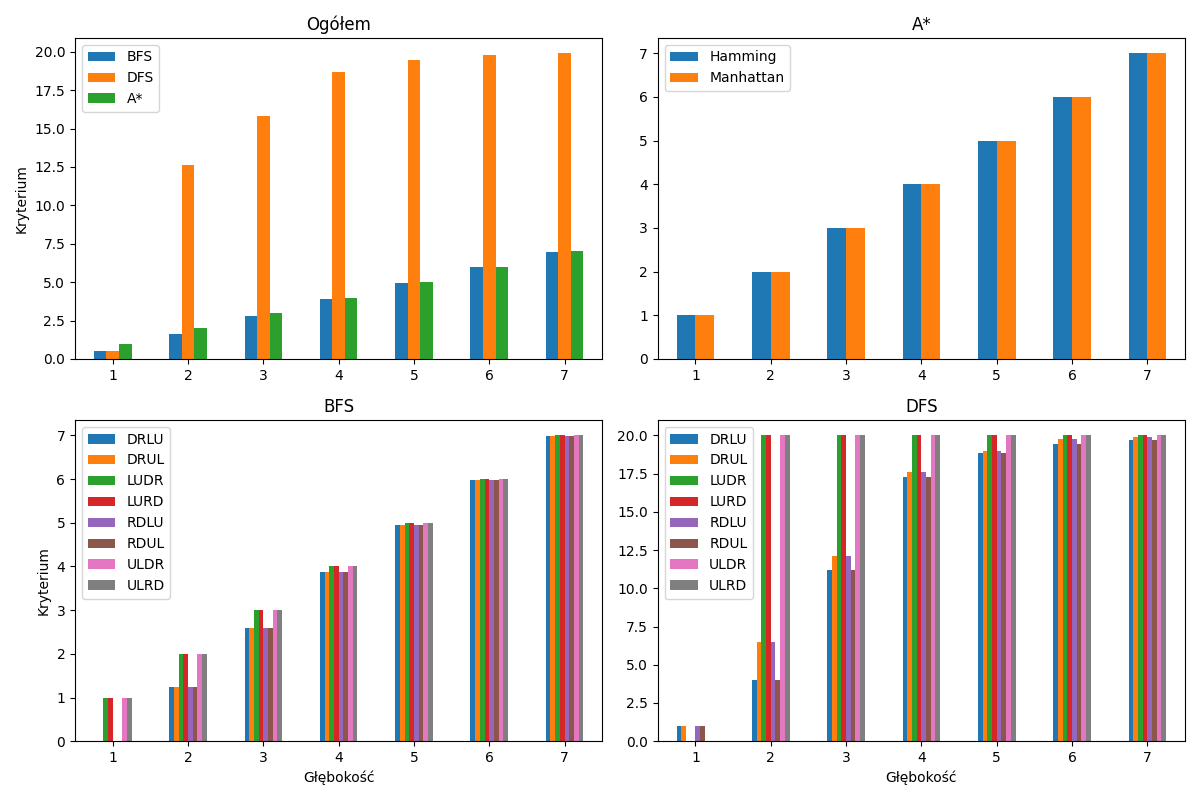
\includegraphics[width=0.9\textwidth]{wyniki_glebokosc.png}
    \caption{Maksymalna osiągnięta głębokość rekursji w zależności od głębokości stanu początkowego.}
\end{figure}

\vspace{0.5cm}
\noindent
\textbf{Informacja o nieznalezionych rozwiązaniach:} \\
W przeprowadzonych testach jedynie dla algorytmu przeszukiwania w głąb (DFS) pojawiły się układy, dla których nie udało się uzyskać rozwiązania, niezależnie od wybranego wariantu przeszukiwania sąsiedztwa. Łącznie przeprowadzono \textbf{7434 testy} (z czego 3304 wykorzystywało strageię DFS). Z tej puli poprawnie rozwiązano 7120 układów, jednak w przypadku strategii DFS dokładnie \textbf{314 badanych układów} pozostało nierozwiązanych. Powodem było osiągnięcie założonego limitu głębokości wynoszącego 20. Zestawienie tych wyników prezentuje Tabela \ref{tab:statystyki_rozwiazan}.

\begin{table}[H]
    \centering
    \begin{tabular}{lccc}
        \toprule
        \textbf{Strategia} & \textbf{Łączna liczba testów} & \textbf{Rozwiązane} & \textbf{Nierozwiązane} \\ 
        \midrule
        BFS & 3304 & 3304 & 0 \\ 
        DFS & 3304 & 2990 & 314 \\ 
        A* & 826  & 826  & 0 \\ 
        \midrule
        \textbf{Suma} & \textbf{7434} & \textbf{7120} & \textbf{314} \\ 
        \bottomrule
    \end{tabular}
    \caption{Zestawienie skuteczności algorytmów na podstawie liczby rozwiązanych układów.}
    \label{tab:statystyki_rozwiazan}
\end{table}
\end{document}